% chapters/chapter2/2_7_trajectory.tex
% !TeX root=../../main.tex
\section{برنامه‌ریز مسیر سینماتیکی}
\label{sec:trajectory_planner}

طراحی یک پروفایل حرکتی مطلوب برای هدایت کالسکه، پیش‌نیاز اساسی در کنترل سیستم‌های مکانیکی زیرفعال محسوب می‌شود. در معماری‌های پایه، اعمال ناگهانی خطای موقعیت به سیستم کنترلی در قالب ورودی پله (\lr{Step Input})، به دلیل درخواست نیروی محرک غیرواقع‌بینانه، منجر به اشباع عملگرها، اعمال شوک‌های مکانیکی به سازه و خروج دینامیک آونگ از محدوده خطی پایدار می‌شود. برای غلبه بر این محدودیت ساختاری، موقعیت هدف باید در قالب یک مسیر پیوسته و سینماتیکی تولید شود. بدین منظور، از یک برنامه‌ریز مسیر (\lr{Trajectory Planner}) بر مبنای چندجمله‌ای‌های نرم (\lr{S-Curve}) استفاده شده است.

\subsection{ریاضیات و فرمولاسیون مسیر مرجع}
برای تضمین پیوستگی در پروفایل‌های موقعیت، سرعت و شتاب و همچنین جلوگیری از بروز ضربه (\lr{Jerk}) نامتناهی در سیستم، یک چندجمله‌ای مرتبه $5$ برای تولید مسیر حرکتی به کار می‌رود. استفاده از مرتبه $5$، امکان ارضای شش شرط مرزی حیاتی را در ابتدا ($t=0$) و انتهای ($t=T$) مسیر فراهم می‌کند؛ به گونه‌ای که سرعت و شتاب کالسکه در هر دو نقطه دقیقاً برابر صفر باشد. با در نظر گرفتن زمان نرمالایز شده $\tau = t/T$، فرم کلی چندجمله‌ای به شکل $s(\tau) = c_0 + c_1\tau + c_2\tau^2 + c_3\tau^3 + c_4\tau^4 + c_5\tau^5$ تعریف می‌شود. اعمال شرایط مرزی $s(0)=\dot{s}(0)=\ddot{s}(0)=0$ و $s(1)=1, \dot{s}(1)=\ddot{s}(1)=0$، ضرایب معادله را به صورت یکتا تعیین کرده و مشتقات سینماتیکی آن به فرم زیر استخراج می‌شوند:
\begin{equation}
    s(\tau) = 10\tau^3 - 15\tau^4 + 6\tau^5
\end{equation}
\begin{equation}
    \dot{s}(\tau) = \frac{1}{T} \left( 30\tau^2 - 60\tau^3 + 30\tau^4 \right)
\end{equation}
\begin{equation}
    \ddot{s}(\tau) = \frac{1}{T^2} \left( 60\tau - 180\tau^2 + 120\tau^3 \right)
\end{equation}

زمان کل سفر ($T$) تابعی از قیود فیزیکی سیستم و ماهیت نوسانی بار است. برای حفظ نیروی درخواستی در محدوده ظرفیت نامی موتورها، حداکثر سرعت مجاز ($v_{\max} = 1.0$ متر بر ثانیه) و حداکثر شتاب مجاز ($a_{\max} = 2.0$ متر بر مجذور ثانیه) به عنوان قیود سخت تعریف شده‌اند. با محاسبه نقاط اکسترمم توابع سرعت و شتاب، حداقل زمان لازم برای ارضای این قیود به ترتیب $T_v = \frac{15}{8} \frac{D}{v_{\max}}$ و $T_a = \sqrt{\frac{5.77 D}{a_{\max}}}$ به دست می‌آید که در آن‌ها $D$ مقدار مطلق جابجایی است.

علاوه بر قیود سینماتیکی، یک قید دینامیکی نیز بر اساس دوره تناوب طبیعی آونگ ($T_p = 2\pi\sqrt{l_0/g}$) در نظر گرفته شده است. حصول اطمینان از اینکه زمان مانور حداقل $1.5$ برابر این دوره تناوب ($T_p$) باشد، از تحریک رزونانسی دینامیک نوسانی در جابجایی‌های بسیار کوتاه جلوگیری می‌کند. در نهایت، زمان کل سفر به عنوان بیشینه این سه مقدار انتخاب می‌شود تا تمامی شروط به صورت هم‌زمان ارضا شوند:
\begin{equation}
    T = \max \left( \frac{15}{8} \frac{D}{v_{\max}}, \sqrt{\frac{5.77 D}{a_{\max}}}, 1.5 T_p \right)
\end{equation}

این سازگاری سینماتیکی سبب می‌شود که الگوریتم برای هر کورس حرکتی، پروفایل مستقلی تولید کند. نمودار خروجی این برنامه‌ریز برای دو جابجایی کوتاه ($0.5$ متر) و بلند ($5$ متر) در شکل \ref{fig:trajectory_profiles} ارائه شده است. در این پروفایل‌ها، متغیرهای حالت سیستم به گونه‌ای تنظیم شده‌اند که نمودار اول و دوم به ترتیب بیانگر موقعیت و سرعت کالسکه در طول مسیر هستند. نمودارهای سوم و چهارم نیز نشان‌دهنده زاویه و سرعت زاویه‌ای هدف برای آونگ هستند که به صورت اکید روی مقدار صفر تنظیم شده‌اند تا انتقال بار بدون هیچ‌گونه نوسانی به عنوان مرجع کنترلی به سیستم تحمیل شود.

\begin{figure}[htbp]
    \centering
    \begin{minipage}{0.48\textwidth}
        \centering
        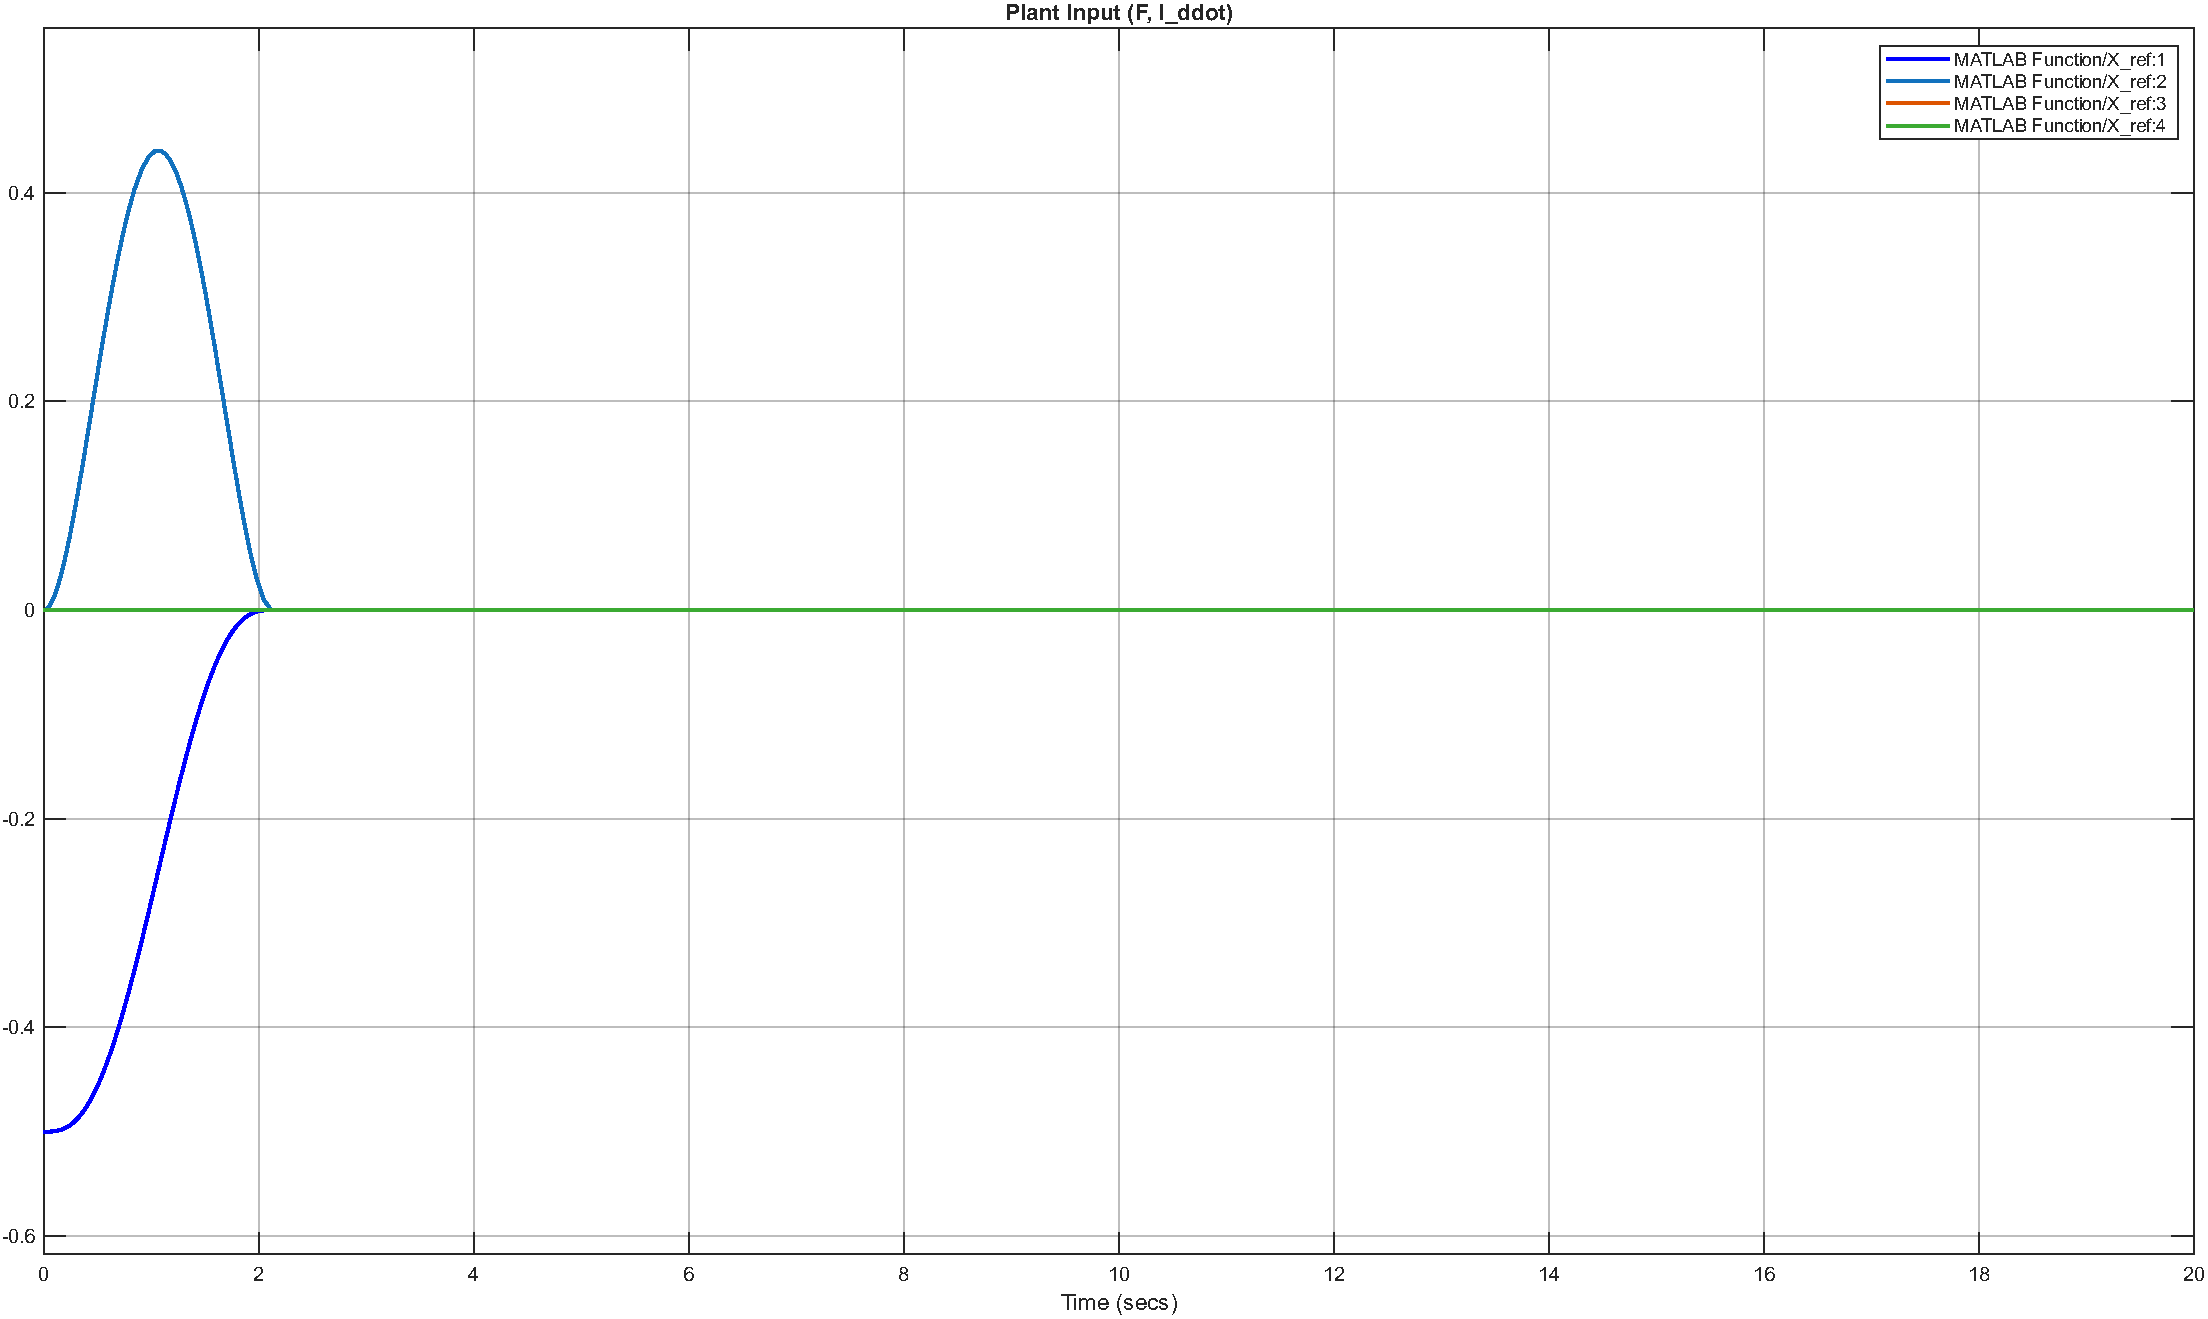
\includegraphics[width=\textwidth]{images/2_LQR_Trajectory/LQR_TRAJ_ref.pdf}
        \vspace{0.2cm}
        \centerline{\footnotesize \rl{(الف) پروفایل سینماتیکی برای جابجایی $0.5$ متر.}}
    \end{minipage}
    \hfill
    \begin{minipage}{0.48\textwidth}
        \centering
        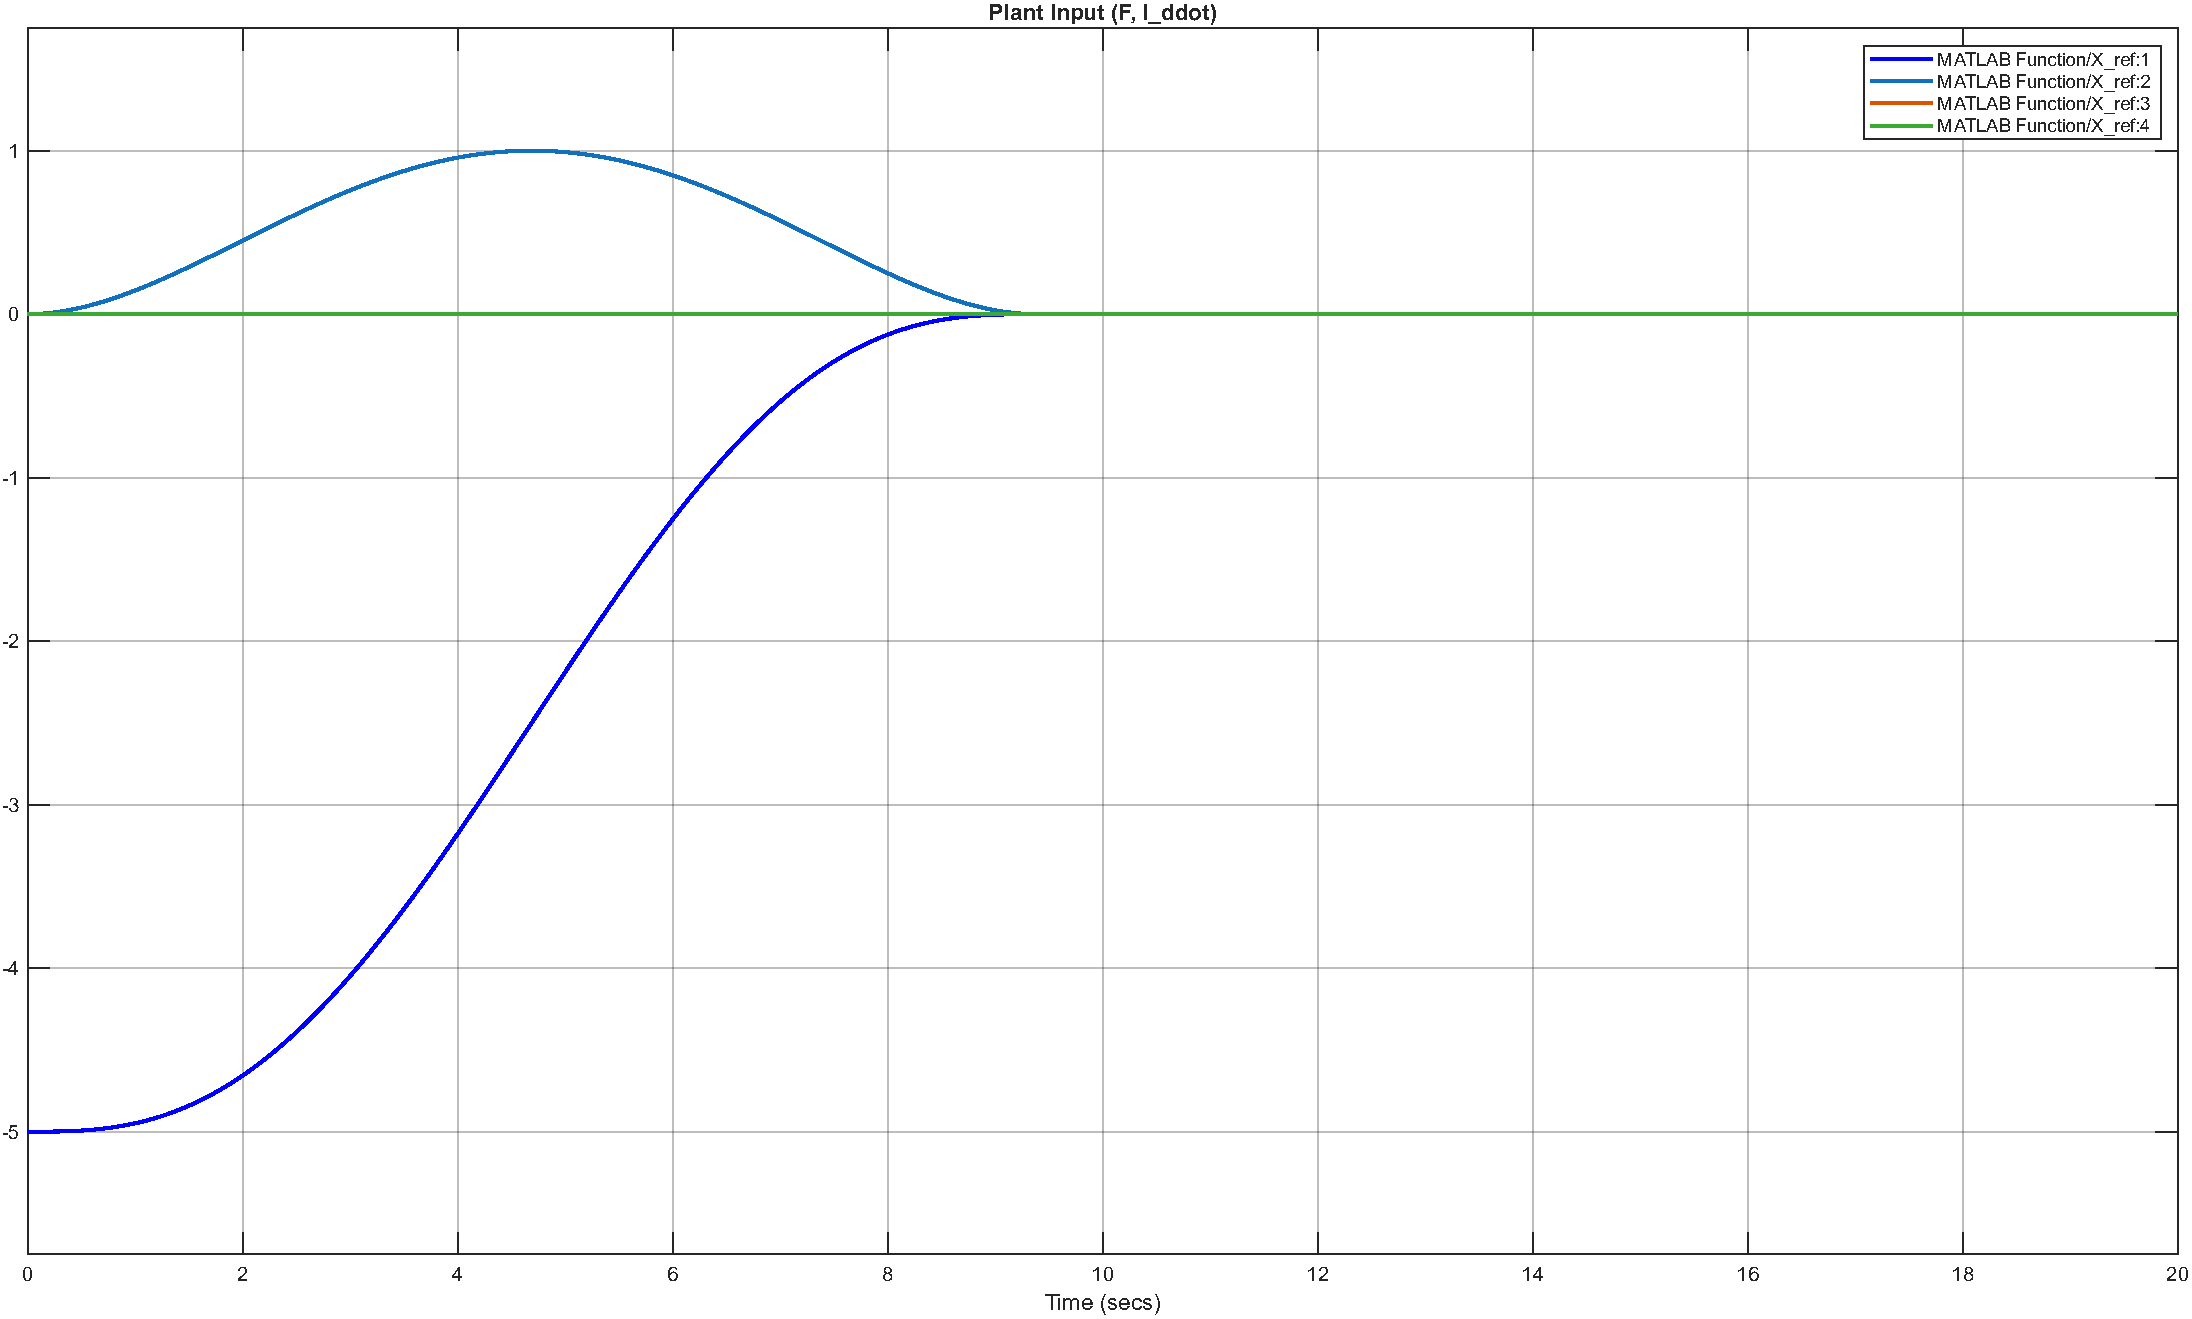
\includegraphics[width=\textwidth]{images/2_LQR_Trajectory/LQR_TRAJ_ref_5.pdf}
        \vspace{0.2cm}
        \centerline{\footnotesize \rl{(ب) پروفایل سینماتیکی برای جابجایی $5$ متر.}}
    \end{minipage}
    \caption{\rl{تطابق خودکار برنامه‌ریز مسیر با مسافت‌های مختلف و تعیین مقادیر مرجع متغیرهای حالت.}}
    \label{fig:trajectory_profiles}
\end{figure}

\subsection{معماری یکپارچه‌سازی در محیط شبیه‌ساز فیزیکی}
نحوه ادغام پروفایل مسیر تولید شده در حلقه کنترل و محیط \lr{Simscape}، وابستگی مستقیمی به ماهیت کنترل‌کننده (خطی یا پیش‌بین) دارد. کدهای توسعه‌یافته جهت پیاده‌سازی این برنامه‌ریز برای معماری‌های مختلف در پیوست \ref{app:matlab_codes} مستند شده‌اند.

\textbf{ادغام مسیر در کنترل‌کننده \lr{LQR}:}
در معماری خطی، کنترل‌کننده فاقد توانایی پیش‌بینی مسیر آینده است. بنابراین، بلوک برنامه‌ریز مسیر (\lr{TrajectoryGenerator\_LQR}) موظف است علاوه بر تولید مقادیر مرجع هندسی لحظه‌ای، یک سیگنال فیدفوروارد تحلیلی ($F_{ff}$) نیز تولید کند. این سیگنال از طریق مدل‌سازی معکوس دینامیکی، نیروی خالص مورد نیاز برای غلبه بر اینرسی کالسکه ($M + m$) و اصطکاک ریل ($b_c$) را در طول مسیر تأمین می‌کند:
\begin{equation}
    F_{ff} = (M + m) a_{ref} + b_c v_{ref}
\end{equation}
همان‌طور که در بلوک‌دیاگرام شکل \ref{fig:lqr_traj_simscape} مشاهده می‌شود، فرمان نهایی عملگر از جمع جبری سیگنال پیش‌خور و سیگنال فیدبک اصلاحی تشکیل می‌شود ($F_{total} = F_{ff} + F_{lqr}$). سیگنال فیدبک صرفاً وظیفه جبران خطاهای لحظه‌ای و سرکوب نوسانات را بر عهده دارد (کد \ref{code:traj_generator_lqr}).

\begin{figure}[htbp]
    \centering
    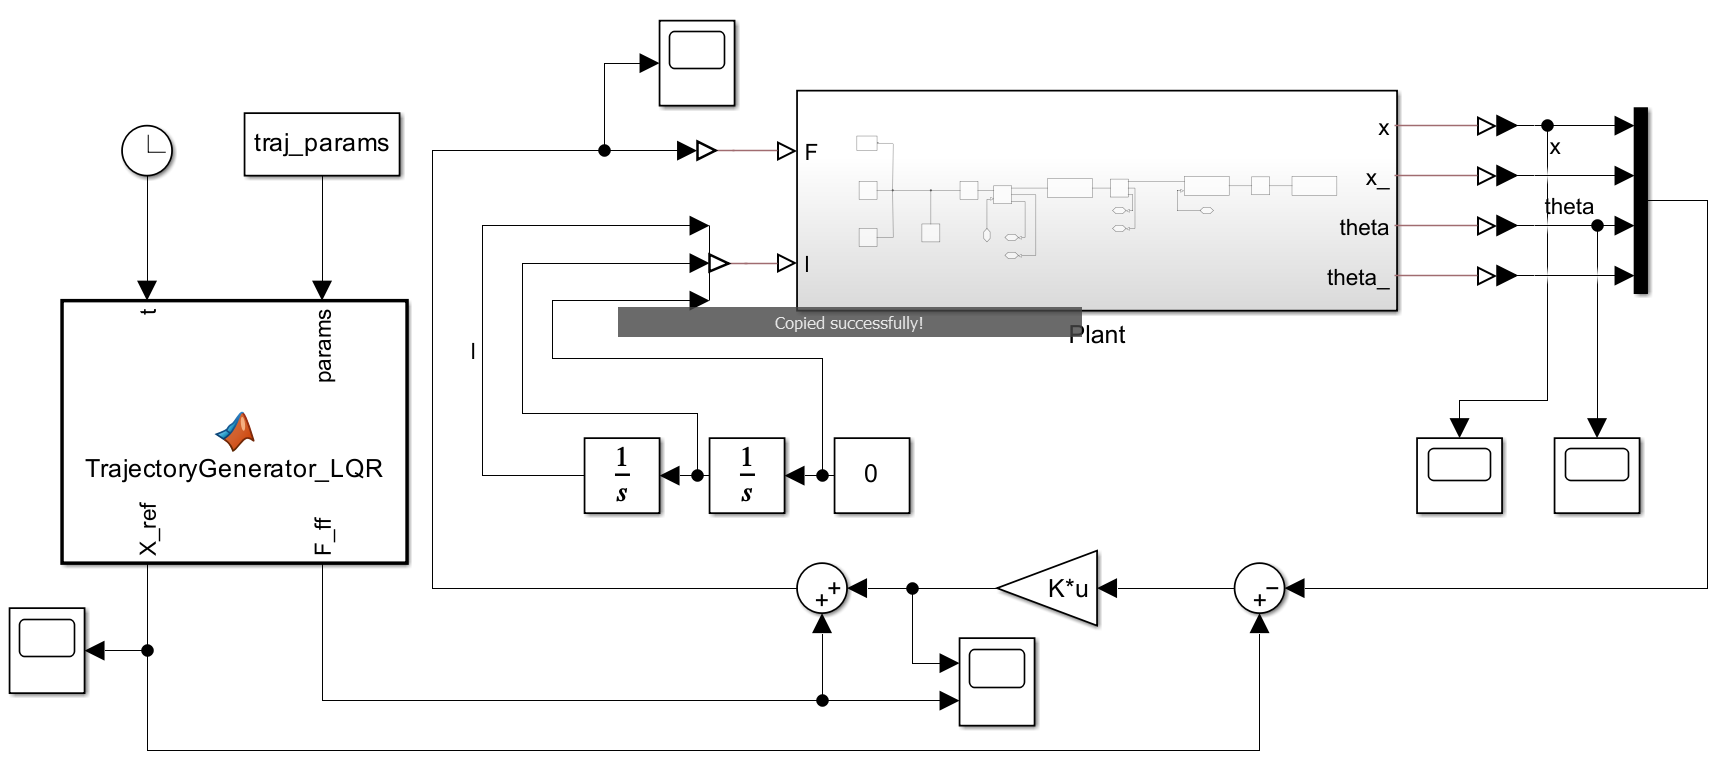
\includegraphics[width=\textwidth]{images/2_LQR_Trajectory/LQR_TRAJ_block_diagram.png}
    \caption{\rl{معماری یکپارچه‌سازی برنامه‌ریز مسیر و سیگنال فیدفوروارد در محیط \lr{Simscape} برای کنترل‌کننده \lr{LQR}.}}
    \label{fig:lqr_traj_simscape}
\end{figure}

\textbf{ادغام مسیر در کنترل‌کننده \lr{NMPC}:}
برخلاف رویکرد کلاسیک، کنترل‌کننده پیش‌بین نیازی به سیگنال فیدفوروارد خارجی و محاسبات دینامیک معکوس ندارد. در این معماری (شکل \ref{fig:nmpc_traj_simscape})، برنامه‌ریز مسیر به گونه‌ای توسعه یافته است تا در هر گام زمانی، آرایه‌ای از نقاط مرجع آینده به طول افق پیش‌بینی ($N_p$) را تولید کرده و به‌صورت یکجا به درگاه مرجع (\lr{ref}) در بهینه‌ساز تزریق کند (کد \ref{code:traj_generator_nmpc}). در این حالت، بردار مرجع شامل $6$ متغیر حالت از جمله طول کابل و مشتقات آن است. حل‌گر غیرخطی \lr{NMPC} با دریافت این مسیر آینده و در اختیار داشتن مدل دینامیکی دقیق سیستم، تلاش کنترلی پیش‌دستانه (\lr{Proactive}) را به‌طور ذاتی درون فرآیند بهینه‌سازی خود محاسبه می‌کند.

\begin{figure}[htbp]
    \centering
    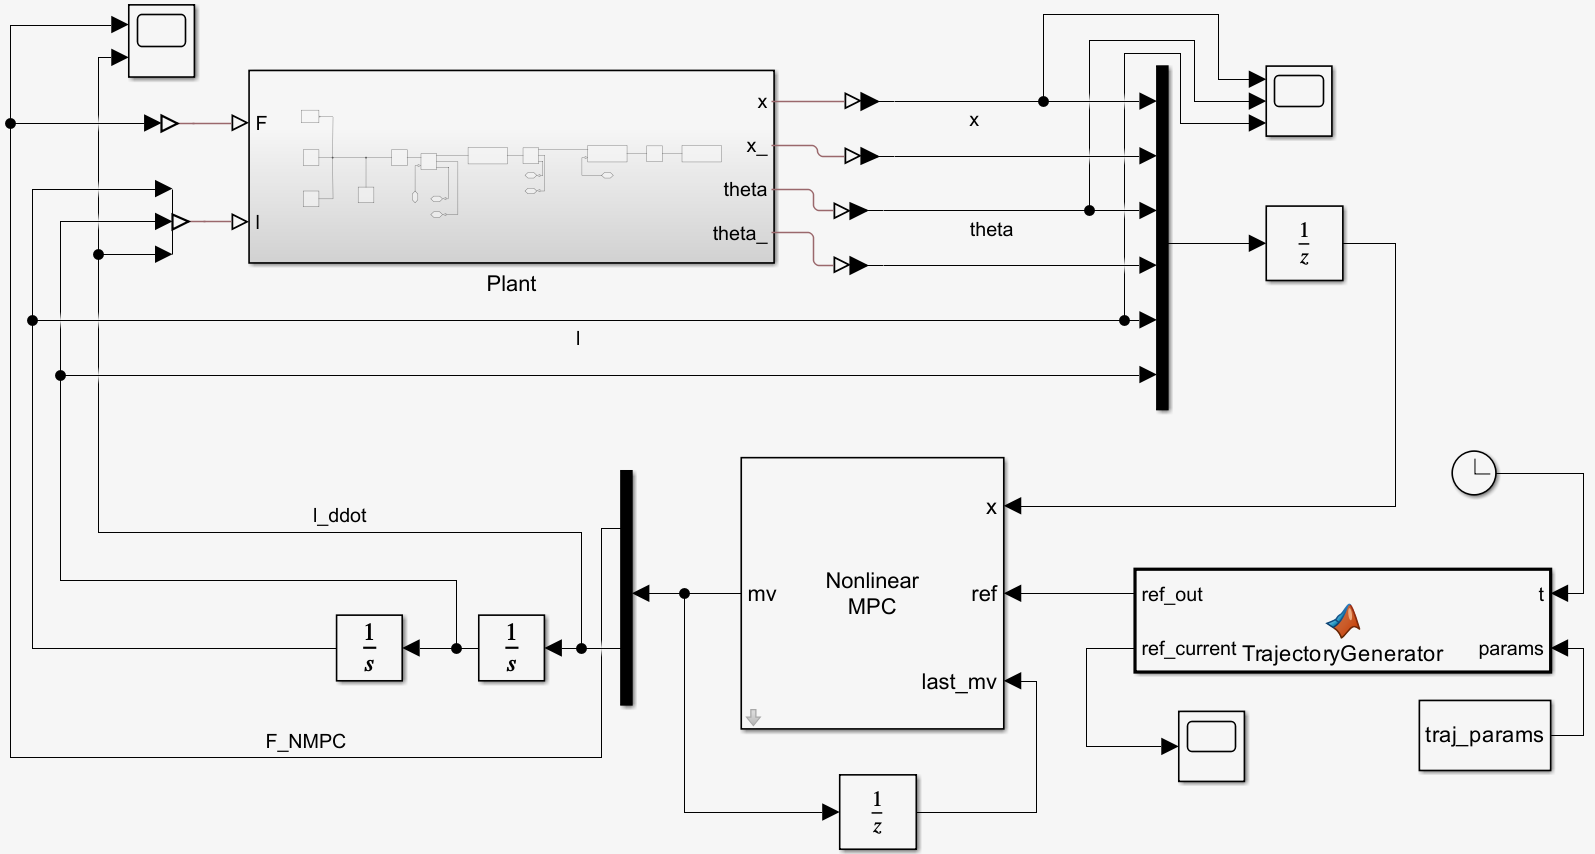
\includegraphics[width=\textwidth]{images/4_NMPC_Trajectory/MPC_TRAJ_block_diagram.png}
    \caption{\rl{معماری یکپارچه‌سازی برنامه‌ریز مسیر مبتنی بر افق پیش‌بینی در محیط \lr{Simscape} برای کنترل‌کننده \lr{NMPC}.}}
    \label{fig:nmpc_traj_simscape}
\end{figure}